\documentclass{ieeeaccess}
\usepackage{cite}
\usepackage{amsmath,amssymb,amsfonts}
\usepackage{algorithmic}
\usepackage{graphicx}

\usepackage{textcomp}
\usepackage{caption}
\usepackage{subcaption}
\usepackage{helvet}  

 \usepackage{comment}
\usepackage{pgfplots}
\usepackage{pgfplotstable}
\pgfplotsset{compat=1.7}
\usepackage{tikz}
\usepackage{tikzscale}
\usetikzlibrary{decorations.markings,decorations.shapes,decorations,arrows,automata,backgrounds,petri,shapes.geometric}  
\usepackage{xcolor} 

\NewSpotColorSpace{PANTONE}
\AddSpotColor{PANTONE} {PANTONE3015C} {PANTONE\SpotSpace 3015\SpotSpace C} {1 0.3 0 0.2}
\SetPageColorSpace{PANTONE}
%\usepackage{tikz}  
%\usepackage{helvet}  
%\usetikzlibrary{decorations.markings,decorations.shapes,decorations,arrows,automata,backgrounds,petri,shapes.geometric}  
%\usepackage{xcolor} 
\newtheorem{Problem}{Problem}
\newtheorem{Definition}{Definition}

\def\BibTeX{{\rm B\kern-.05em{\sc i\kern-.025em b}\kern-.08em
    T\kern-.1667em\lower.7ex\hbox{E}\kern-.125emX}}

\begin{document}
\history{Date of publication xxxx 00, 0000, date of current version xxxx 00, 0000.}
\doi{10.1109/ACCESS.2017.DOI}

\title{On semantic mapping to visualize Knowledge Graphs}
\author{\uppercase{P. Camarillo-Ramirez}\authorrefmark{1},
\uppercase{F. Cervantes-Alvarez\authorrefmark{1}, and L. F. Guti\'{e}rrez-Preciado}.\authorrefmark{1}}
\address[1]{Western Institute of Technology and Higher Education, Tlaquepaque, Jalisco 45601 Mexico (ng724453@iteso.mx;fcervantes@iteso.mx;lgutierrez@iteso.mx)}

\tfootnote{This work was supported in part by the  National Council of 
Science and Technology of Mexico through grant 498322}

\markboth
{Author \headeretal: Preparation of Papers for IEEE TRANSACTIONS and JOURNALS}
{Author \headeretal: Preparation of Papers for IEEE TRANSACTIONS and JOURNALS}

\corresp{Corresponding author: P. Camarillo-Ramirez (e-mail: ng724453@iteso.mx)}

\begin{abstract}
Knowledge Graphs (KGs) are one of the most novel technologies used to
improve search engines and support
decision making in the life sciences since they structure information in graph form
by encoding concepts as nodes, and the semantics of the relationship
among concepts as edges. The analysis of these kind of structures calls
for an effective strategy to visualize them. However, the increasing
size of KGs makes the exploring process a big challenge.
A semantic map is a visual representation of related concepts that helps humans
in the learning process. In this work, we propose to generate a simplified visual
representation of a KGs by generating a semantic maps. We used the affinity propagation
algorithm to find the \textit{related} concepts in KGs. We used different semantic similarity
measures to compute the groups of related concepts.


\end{abstract}

\begin{keywords}
Knowledge graphs; Knowledge graphs visualization; Semantic similarity; Semantic mapping; Big Data;
\end{keywords}

\titlepgskip=-15pt

\maketitle

\section{Introduction}
\label{sec:introduction}

Knowledge Graphs (KGs) are considered one of the emerging technologies 
associated with Big Data that are leading the digital ecosystems by 
providing a mechanism to obtain valuable information from heterogeneous 
digital means \cite{Panetta19}. KGs encode knowledge from different sources
into structured documents that can be interpreted by machines. Recently, 
academic and private organizations have constructed KGs, such as YAGO 
\cite{suchanek2007yago}, DBPedia \cite{auer2007dbpedia}, Freebase 
\cite{Freebase08}, NELL\cite{NELL10}, Google Knowledge Graph 
\cite{GoogleKG12}, Microsoft Satori \cite{Satori13}, Facebook Entity
Graph \cite{Facebook13}, and Wikidata \cite{Wikidata14}, which contain
millions of entities and billions of relationships. The main applications 
of KGs include the enhancement of search engines like Google \cite{GoogleKG12}
or Bing \cite{Satori13} as well as question answering and decision support
in the life sciences \cite{Belleau08,Ruttenberg09,Momtchev09}. 

Considering the continuous increase in size of these graphs, the goal of 
visual graph analysis become uncertain due to a lacking ability to observe 
details from the information presented. The visual data exploration is considered as a
hypothesis-generator process by allowing users to gain a deep understanding 
of the data, and thus come up with a new hypothesis thought visualization software
tools\cite{keim2001visual}. On the other hand, semantic mapping is a technique widely used to understand
new concepts which consists of a categorical structuring of information 
in a graphic form \cite{johnson1986semantic}, hence getting an effective visual
representation of a KG is crucial. 

In this paper, we hypothesize 
that semantics maps are useful to visualize the high level of abstraction of 
a KG. To generate effective semantic maps it is necessary to compute 
how similar are two concepts in the KG. The main challenge to build a semantic map
from a KG is to compute the groups of concepts based on their 
semantic similarity. In Unsupervised Learning, clustering algorithms classify data into
one or more classes depending on a similarity or distance measure \cite{SCHAEFFER200727}. In
graph structures, clustering process is aimed to group vertices, therefore if we apply a
clustering algorithm to the data set of concepts in the KG, we would have the groups of
concepts we need to build a semantic map. However, the clustering algorithms depends on a
\textit{appropiate} similarity or distance measure. The semantic similarity is a metric used
in Natural Processing Language (NPL) and Information Retrieval (IR) areas \cite{HOVY20132} that
represents how related are two concepts based on their hierarchical 
relations \cite{resnik1995using}, \cite{turney2010frequency}. Recently, Zhu and Iglesias
\cite{ZhuIglesias2017} proposed a the wpath similarity metric for KGs that combines 
the structure of the semantic network and the information content (IC) of concepts to 
compute the semantic similarity between concepts in KGs.

The main contributions of this work include:
\begin{enumerate}
    \item The method to generate a similarity matrix from a KG.
    \item The strategy to generate a simplified visual representation 
    of a KGs through semantic maps.
    \item The experiments that validates the proposed method and shows the
    obtained semantic maps.
\end{enumerate}

The rest of this paper is structured as follows. In the Section \ref{sec:related},
we review the related work associated with knowledge graph visualization, graph 
clustering, semantic similarly, and semantic mapping. In Section \ref{sec:Method}, we 
describe the method we used to build semantic maps using clustering algorithms. Next in 
Section \ref{sec:results}, a set of experiments showing the generated semantic maps for 
selected data sets from DBPedia.


\section{Related work}
\label{sec:related}
This section is focused on describing the most relevant works associated with
the problem of graph summarization and its relevance to the visual data
exploration area.


\subsection{Graph visualization}

Recent applications have
proven useful for large graph visualizations to understand
different phenomena, such as Bitcoin transactions 
\cite{mcginn2016visualizing} and online discussions
\cite{molina2017improving}. For big knowledge graphs, it is necessary a
distributed implementation of the layout algorithms to improve the time 
needed to generate the visual representation \cite{gomez2018visualizing}. 

Recent works \cite{6787141,1703364,8801911} have shown that visualizing a 
simplified version of a large graph is an adequate alternative. For instance, \cite{Tasnim2020} 
visualizing a summarized graph can be useful when it is not possible to 
implement a distributed solution to render a large graph. Functional
summaries were proposed by the bioinformatics community to obtain a 
concise and interpretable representation of a Protein-Protein Interaction (PPI)
network \cite{Seah12}. These functional summaries are high level abstraction
maps built from a knowledge base.


In the context of data mining, summarization is the process of facilitating 
the identification of meaningful data. In this work, our focus is on the
study of the summarization for networked data, also known as networks or
graphs. The applications of graph summarization include reduction of data
volume and storage, speedup of graph algorithms and queries, interactive
analysis support, and noise elimination \cite{liu2018graph}. 


Recent works have been proposed to summarize large graphs in order to enable an efficient 
visualization of their content. In \cite{OntoVis}, Shen et al. propose a visual 
analytics tool called OntoVis, which performs both structural and semantic abstractions to offer
a summarized version of a large graph to visualize a simplified version of the graph. Another
related work is presented in \cite{koutra2014vog}, which describes the VoG (Vocabulary-based
summarization of Graphs) algorithm to summarize and understand large graphs by constructing
and visualizing subgraph-types, such as starts, cliques, and chains. The visual abstraction
presented in \cite{8801911}, transforms geo-tagged social media data into high-dimensional
vectors by utilizing a doc2vec model. In \cite{Koutra2019}, the authors focus on 
summarizing KGs by taking advantage of individual interests to generate personalized
knowledge graph summaries.

Regardless of the application, one of the main challenges of graph summarization is defining
which data is of interest. Every summarization strategy depends on selecting an interest
criteria to extract meaningful information \cite{liu2018graph}. However, to achieve a concise
definition of \textit{interesting} is not an easy task. For example, the FUSE algorithm \cite {Seah12} 
proposes a profit maximization model that seeks to find a summary by maximizing information
profit under a budget constraint. On the other hand, VoG \cite{koutra2014vog} exploits
the Minimum Description Length (MDL) principle aimed at identifying the best subgraphs
by choosing those which save most bits. In the case of semantic abstraction proposed in
\cite{8801911}, a dual-objective blue noise sampling model is utilized to select a subset
of social media data items supporting the spatial distribution and semantic correlation for
the resulting simplified geographical visualization. In the personalized summaries from
KGs described in \cite{Koutra2019}, the criteria to decide which information is \textit{interesting}
for each user is determined by reviewing the users' query history.

In the taxonomy of graph summarization algorithms
proposed by Koutra et al. \cite{liu2018graph}, the authors include
two families of graph summarization techniques that are based on the 
network type: static and dynamic. In this work, we consider the summarization
of static graphs.


\subsection{Visual Data Exploration of knowledge graphs}
The idea behind the visual data exploration process is to present the data
in some visual form, allowing users to draw conclusions of the analyzed
phenomena \cite{keim2001visual}. This process, also known as the "information
seeking mantra", follows three steps: overview, zoom and filter, and 
details-on-demand \cite{Shneiderman96}. In this context, ontologies are considered
one of the most relevant data visualization techniques. In the field of 
computer science, an ontology is a model for describing the world that consists
of a set of types, properties, and relationship types \cite{Garshol2004MetadataTT}
and by providing an initial attempt to visualize linked data.

In regard to visual exploration of KGs, challenges include context adaptation,
users \cite{Koutra2019}, data heterogeneity \cite{OntoVis,6787141,1703364}, 
supporting diverse analysis tasks (query, combination, filtering, etc.), 
and performance \cite{gomez2018visualizing}. In this study, the summarization
technique implemented is aimed at enabling an effective visual representation
of a large knowledge graph.

Some works associated with visual representation of networks or KGs
take into account the data exploration objectives \cite{ARCHAMBAULT20131044, 8801911}.
In contrast, other approaches are focused on evaluating the \textit{usability} of software
tools instead of evaluating the visual representation to fulfil visual data exploration
tasks \cite{UsabilityMeasurement2006, ISO9241112018, Camarillo20}. 

\section{Methodology}
\label{sec:Method}

In this section, the summarization problem is formally define as well as
some concepts needed to understand the FUSE algorithm. Then, a list the 
changes for adapting the FUSE algorithm to different biology domains is 
presented.

\subsection{Preliminaries}

A \textbf{graph} $G$, also known as network, is an abstract data type consisting
of a finite set of vertices (nodes) $V$, a finite set of links (edges) $E$ (disjoint
from $V$), and an \textit{incidence function} $\psi_{G}$ that associates with each
edge of $G$, an unordered pair of vertices of $G$. If $e \in E$ and $u, v \in V$ such that 
$\psi_{G}(e) =  uv$, then $e$ is said to join $u$ and $v$; the vertices $u$ and $v$ are
called the \textit{ends} of $e$ \cite{bondy1976graph}.

When a graph has attributes associated to nodes or edges, it can be
considered a knowledge graph. A \textbf{knowledge graph}
$KG=(E,R,T)$ consists of a set of entities $E$, a set of relations 
$R$, and a set of triples $T \subseteq E \times R \times E^{1}$. A
triple connecting entities $e_{i},e_{j} \in E$ with relation $r_{k} 
\in R$ is denoted $x_{ijk} = (e_{i},r_{k},e_{j})$ \cite{Koutra2019}. 
In other words, KGs consist in a collection of facts formed 
by $<subject,predicate,object>$. These collections are typically
represented in languages, such as RDF (Resource Description
Framework) \cite{RDF} and OWL (Ontology Web Language) \cite{OWL}.

% TODO: Agregar teoria de moleculas rdf 
\subsection{Functional summarization for Knowledge graphs}

The core of this paper lies in summarizing knowledge graphs by obtaining
functional summaries. The formal definition of a functional cluster
is:

\begin{Definition}
\textbf{Functional Cluster} \\
Let $ V (a_{i}) \subseteq V$ denote the set of
vertices in $G$ such that $v \in V (a_{i})$ if and only 
$ \Delta_{v} [a_{i}(v)] = 1$. The functional cluster of  $a_{i} \in \Delta$, 
denoted by $C(a_{i}) \subseteq G$, is the subgraph of $G$ that is induced 
by $V (a_{i})$.

\end{Definition}

Table \ref{tab:Symbols} enumerates the symbols utilized in the rest of this section.

\begin{table}[!ht]
\caption{Symbols associated with the summarization process}
\label{tab:Symbols}
\centering
\begin{tabular}{r|l}
\hline
\bfseries Symbol & \bfseries Meaning \\ \hline \\
$C(u)$ & Functional cluster \\
$KG$ & Input knowledge graph \\
$\Theta_{KG}$ & Functional summary of $KG$\\
$D$ & Directed acyclic graph (DAG) from an Ontology \\
$\Delta$ & Topological sort of $D$ \\
$k$ & Input parameter to specify the summary level \\
$b$ & Information budget assigned to every node $i \in V$ \\
$d$ & Penalization parameter introduced to penalize redundancy. \\
& Typically  $0 \leq d \leq 10$ \\
$\beta$ & Significance cut-off parameter used to \\ 
& associate a pair of functional clusters \\
$\Psi^{C(u)}$ & Structural knowledge value \\
$S_{\Delta}$ & Set of functional clusters induced from $\Delta$.\\
$S$ & Set of higher-order functional clusters \\
$\Delta_{v}[a_{i}(v)]$ & Term association vector of $v \in V$ \\
$F$ & Set of edges that links the functional clusters \\
$P_{i}$ & Probability density function of observing $o_{uv}$ or more \\
& number of interactions between C(u) and C(v). \\
$\alpha$ & The bijection $\alpha : 1, 2, \dots ,m \leftrightarrow S$ is an ordering of S. \\
\hline
\end{tabular}
\end{table}

The functional summarization problem consists of finding $\Theta_{KG}$
that represent the underlying PPI subject to a summary complexity constraint.
This work is aimed at adapting the FUSE algorithm to use a knowledge graph instead of
a PPI. To find a functional summary, a profit maximization model is proposed to
obtain $\Theta_{KG} = (S, F, P_{i}, \alpha)$ by maximizing information under a
budget constraint. In the original problem, every protein $i \in V$ is assigned
a non-negative \textit{information budget} $b$, which stands for the information
constraint. In our proposal, this information budget is associated to every node in
the knowledge graph that needs to be summarized. Every functional cluster $C(u) \in S_{\Delta}$
is assigned a non-negative \textit{structural information value} $\Psi^{C(u)}$, which
represents the amount of structural information contained within the functional
subgraph. The formula to compute the structural information value is:

\begin{equation}
\label{eqn_coverage}
\Psi^{C(u)} = \frac{\sum_{i,j \in C(u)} E_{ij}}{C(u)}
\end{equation}

In this work, this structural information value is the amount of structural
\textit{knowledge} contained in the functional subgraph of $KG$. When a functional
cluster $C(u)$ is added to the summary, for every node $i \in V(u)$, a portion of $b$ 
is taken out and added to summary functional information gain.

\begin{Definition}
\textbf{Functional summary of a Knowledge Graph} \\
Let $K_{i}$ be a set of functional clusters such that $C(u) \in K_{i}$ if and only if
$i \in C(i)$. For every $C(u) \in S_{\Delta}$, let $\Psi^{C(u)}$ be the structural knowledge
information value of $C(u)$. Given a knowledge graph $KG = (E,V,T)$ and input parameters
$b, d$, and $k$, the \textit{functional summarization problem adapted to KGs} generates a
\textit{k-cluster} FSKG $\Theta_{KG} = (S, F, P_{i}, \alpha)$ subject to $\vert S \vert = k$.

\end{Definition}

\section{Experimental results}
\label{sec:results}
The adaptation of the FUSE algorithm proposed in this work is implemented in Python and Java
programming languages. Results presented in this section correspond to experiments that were run on 
a machine with 2 GHz Quad-Core Intel Core i7 processor, 8 GB 1600 MHz DDR3, a graphics
card Intel Iris Pro with 1536 MB, and 250 GB of flash storage. The software tool utilized to
perform the efficiency evaluation is WebVOWL \footnote{http://www.visualdataweb.de}.

\subsection{Evaluation metrics}

The use of heatmaps works as a high-level view of the similarity matrix to
visualize which groups of concepts are more likely to be clustered together \cite{NGUYEN201495}. 

To evaluate the quality of the obtained summaries, the data
mining literature offers two metrics: coverage and redundancy. The
coverage metric is the ratio of the total number of annotated nodes in the
summary over the total number of annotated nodes in the input knowledge 
graph (Eq 1). The redundancy metric is the average number of functional clusters 
that each node belongs to. This is an indicator of the amount of cluster overlap in 
the summary (Eq. 2)

\begin{equation}
\label{eqn_coverage}
coverage(\Theta) = \frac{\lvert \cup_{C(u) \in S_{\Theta}}  V(u)
\rvert}{\lvert \cup_{C(u) \in S_{\Delta}} V(u)\rvert}
\end{equation}

\begin{equation}
\label{eqn_redundancy}
redundancy(\Theta) = \frac{\sum_{C(u) \in S_{\Theta}} V(u) }
{\lvert \cup_{C(u) \in S_{\Theta}}  V(u)
\rvert} 
\end{equation}

Other well-known statistical measures to indicate accuracy and completeness are
precision and recall. These measures are defined as follows:

\begin{equation}
\label{eqn_precision}
precision = \frac{TP}{TP + FP}
\end{equation}

\begin{equation}
\label{eqn_recall}
recall = \frac{TP}{TP + FN}
\end{equation}

Neighborhood similarity. Neighborhood of an entity $e \in V$ is 
defined as the set of relation-entity pairs $N(e)$ whose entities
are at one-hop distance of $e$, i.e.,

\begin{equation}
    N(e) = \{(r, e_{i})|(e,r,e_{i}) \in E \}
\end{equation}

In the context of knowledge graph functional summarization, if a
cluster $C(i)$ is assigned with the function $i$, then any term $t \in C(i)$
that is not annotated with $i$ or its descendants is considered a false positive (FP).
If $t \in C(i)$ is annotated with $i$ or descendants, it is a true positive (TP). On the other
hand, a term $t \in V$ that is annotated with $i$ but not in $C(i)$ is considered a false negative (FN).
Nodes from knowledge graph with no cluster associated are not taken into consideration to compute these metrics.

\subsection{Summarizing financial networks: a case study}
In order to validate our initial hypothesis that proposes using the FUSE algorithm to obtain a simplified
version of networks for a different domain than biology, we used the four KG from the financial sector
obtained from the open network repository \cite{nr} (See Table \ref{tab:networks}).

\begin{table}[!ht]
\caption{Datasets of financial and economic sector}
\label{tab:networks}
\centering
\begin{tabular}{|l|l|l|l}
\hline
\bfseries Dataset & \bfseries \# nodes & \# \bfseries edges \\
beacxc & 497 & 50K \\ 
beaflw & 507 & 53K \\
beause & 507 & 44.2K \\
mahindas & 1.3K & 7.6K \\
\hline
\end{tabular}
\end{table}

The ontology utilized to validate the adaptation of the FUSE algorithm 
the Financial Industry Business Ontology  (FIBO) which describes the
sets of entities that are of interest in  financial business applications
\cite{FIBO}. FIBO is developed as an ontology in  the Web Ontology 
Language (OWL) (Table \ref{tab:fibo}).

\begin{table}[!ht]
\caption{Structural information of FIBO}
\label{tab:fibo}
\centering
\begin{tabular}{|l|l|l|l}
\hline
\bfseries Metric & \bfseries Value \\
Axioms & 6498 \\
Logical axiom count & 1530 \\
Declaration axioms count & 889 \\
Class count & 403 \\
Object property count & 266 \\
Data property count & 85 \\
Annotation Property count & 96 \\
\hline
\end{tabular}
\end{table}



We begin with the quality analysis of the functional clusters that were obtained
using the adapted FUSE algorithm. Quality results obtained from the modified FUSE algorithm
are compared with the graph based $k-means$ algorithm \cite{GraphMinning:2013}. Figure 
\ref{fig:ClustersQuality} plots the values of precision and recall for every summarized network with
different summary levels. The user-defined parameters were used with the following
values $\beta = 0.0.1$, $b = 3$, and $d = 0$. The precision values
for all summarized graphs were above 60\%. In contrast, recall values
decreased when the summary level increased.

Figure \ref{fig:ClustersQualityClassical} shows the values for precision and recall
metrics using the k-means algorithm. The kernel matrix associated with every network analyzed
is generated by using the Laplacian Kernel and the number of centroids is 5.




\subsection{Efficiency evaluation of functional summaries}
To compute the visual representation efficiency of clusters
generated by the modified FUSE algorithm, we appled the methodology
proposed in \cite{Camarillo20}. This task-based evaluation methodology 
consists of two phases: establishing the context of use and analyzing
the exploratory data analysis tasks under study.



\subsubsection{Establishing the context of use for network visualization user interface}
\textbf{Generate the network to be visualized.} Network \textit{mahindas} is selected to perform the
efficiency assessment. The summary level is set at $k = 5$. The visualization of
the generated summary is shown in Figure \ref{Fig:Vis_1}.

\begin{figure}[h!]
    \centering
      %%%%%%%%%%%%%%%%%%%%%%%%%%%%%%%%%%%%%%%%%%%%%%%%%%%%%%%%%%%%%%%%%%%%
 %        Generated with the experimental alpha version of the TeX exporter of WebVOWL (version 1.1.3) %%% 
 %%%%%%%%%%%%%%%%%%%%%%%%%%%%%%%%%%%%%%%%%%%%%%%%%%%%%%%%%%%%%%%%%%%%

 %   The content can be used as import in other TeX documents. 
 %   Parent document has to use the following packages   
 %   \usepackage{tikz}  
 %   \usepackage{helvet}  
 %   \usetikzlibrary{decorations.markings,decorations.shapes,decorations,arrows,automata,backgrounds,petri,shapes.geometric}  
 %   \usepackage{xcolor}  

 %%%%%%%%%%%%%%% Example Parent Document %%%%%%%%%%%%%%%%%%%%%%%
 %\documentclass{article} 
 %\usepackage{tikz} 
 %\usepackage{helvet} 
 %\usetikzlibrary{decorations.markings,decorations.shapes,decorations,arrows,automata,backgrounds,petri,shapes.geometric} 
 %\usepackage{xcolor} 

 %\begin{document} 
 %\section{Example} 
 %  This is an example. 
 %  \begin{figure} 
 %    \input{<THIS_FILE_NAME>} % << tex file name for the graph 
 %    \caption{A generated graph with TKIZ using alpha version of the TeX exporter of WebVOWL (version 1.1.3) } 
 %  \end{figure} 
 %\end{document} 
 %%%%%%%%%%%%%%%%%%%%%%%%%%%%%%%%%%%%%%%%%%%%%%%%%%%%%%%%%%%%%%%%%%%%

\definecolor{imageBGCOLOR}{HTML}{FFFFFF} 
\definecolor{owlClassColor}{HTML}{AACCFF}
\definecolor{owlObjectPropertyColor}{HTML}{AACCFF}
\definecolor{owlExternalClassColor}{HTML}{AACCFF}
\definecolor{owlDatatypePropertyColor}{HTML}{99CC66}
\definecolor{owlDatatypeColor}{HTML}{FFCC33}
\definecolor{owlThingColor}{HTML}{FFFFFF}
\definecolor{valuesFrom}{HTML}{6699CC}
\definecolor{rdfPropertyColor}{HTML}{CC99CC}
\definecolor{unionColor}{HTML}{6699cc}
\begin{center} 
\resizebox{\linewidth}{!}{
\begin{tikzpicture}[framed]
\clip (-301.86869909601575pt , 606.3607158180557pt ) rectangle (1913.0135603824654pt , -1765.0871007588225pt);
\tikzstyle{dashed}=[dash pattern=on 4pt off 4pt] 
\tikzstyle{dotted}=[dash pattern=on 2pt off 2pt] 
\fontfamily{sans-serif}{\fontsize{12}{12}\selectfont}
 
\tikzset{triangleBlack/.style = {fill=black, draw=black, line width=1pt,scale=0.7,regular polygon, regular polygon sides=3} }
\tikzset{triangleWhite/.style = {fill=white, draw=black, line width=1pt,scale=0.7,regular polygon, regular polygon sides=3} }
\tikzset{triangleBlue/.style  = {fill=valuesFrom, draw=valuesFrom, line width=1pt,scale=0.7,regular polygon, regular polygon sides=3} }
\tikzset{Diamond/.style = {fill=white, draw=black, line width=2pt,scale=1.2,regular polygon, regular polygon sides=4} }
\tikzset{Literal/.style={rectangle,align=center,
font={\fontsize{12pt}{12}\selectfont \sffamily },
black, draw=black, dashed, line width=1pt, fill=owlDatatypeColor, minimum width=80pt,
minimum height = 20pt}}

\tikzset{Datatype/.style={rectangle,align=center,
font={\fontsize{12pt}{12}\selectfont \sffamily },
black, draw=black, line width=1pt, fill=owlDatatypeColor, minimum width=80pt,
minimum height = 20pt}}

\tikzset{owlClass/.style={circle, inner sep=0mm,align=center, 
font={\fontsize{12pt}{12}\selectfont \sffamily },
black, draw=black, line width=1pt, fill=owlClassColor, minimum size=101pt}}

\tikzset{anonymousClass/.style={circle, inner sep=0mm,align=center, 
font={\fontsize{12pt}{12}\selectfont \sffamily },
black, dashed, draw=black, line width=1pt, fill=owlClassColor, minimum size=101pt}}

\tikzset{owlThing/.style={circle, inner sep=0mm,align=center,
font={\fontsize{12pt}{12}\selectfont \sffamily },
black, dashed, draw=black, line width=1pt, fill=owlThingColor, minimum size=62pt}}

\tikzset{owlObjectProperty/.style={rectangle,align=center,
inner sep=0mm,
font={\fontsize{12pt}{12}\selectfont \sffamily },
fill=owlObjectPropertyColor, minimum width=80pt,
minimum height = 25pt}}

\tikzset{rdfProperty/.style={rectangle,align=center,
inner sep=0mm,
font={\fontsize{12pt}{12}\selectfont \sffamily },
fill=rdfPropertyColor, minimum width=80pt,
minimum height = 25pt}}

\tikzset{owlDatatypeProperty/.style={rectangle,align=center,
fill=owlDatatypePropertyColor, minimum width=80pt,
inner sep=0mm,
font={\fontsize{12pt}{12}\selectfont \sffamily },
minimum height = 25pt}}

\tikzset{rdfsSubClassOf/.style={rectangle,align=center,
font={\fontsize{12pt}{12}\selectfont \sffamily },
inner sep=0mm,
fill=imageBGCOLOR, minimum width=80pt,
minimum height = 25pt}}

\tikzset{unionOf/.style={circle, inner sep=0mm,align=center,
font={\fontsize{12pt}{12}\selectfont \sffamily },
black, draw=black, line width=1pt, fill=unionColor, minimum size=25pt}}

\tikzset{disjointWith/.style={circle, inner sep=0mm,align=center,
font={\fontsize{12pt}{12}\selectfont \sffamily },
black, draw=black, line width=1pt, fill=unionColor, minimum size=20pt}}

\tikzset{owlEquivalentClass/.style={circle,align=center,
font={\fontsize{12pt}{12}\selectfont \sffamily },
inner sep=0mm,
black, solid, draw=black, line width=3pt, fill=owlExternalClassColor, minimum size=101pt,
postaction = {draw,line width=1pt, white}}}

\draw [black, dotted ,line width=2pt] plot [smooth] coordinates {(481.7254758030043pt, -677.4906834946615pt) (455.1354480320594pt, -790.2357052506695pt)  (428.5454202611145pt, -902.9807270066776pt)};
\node[triangleWhite, rotate=-193.27033080241242] at (430.0779113769531pt, -896.4827270507812pt)   (single_marker0) {};
 \draw [black, dotted ,line width=2pt] plot [smooth] coordinates {(167.88009677736733pt, -1080.9728252814605pt) (269.69431814407784pt, -1028.481146731551pt)  (371.50853951078835pt, -975.9894681816417pt)};
\node[triangleWhite, rotate=-62.72568917253612] at (366.08819580078125pt, -978.7839965820312pt)   (single_marker1) {};
 \draw [black, dotted ,line width=2pt] plot [smooth] coordinates {(-83.05532248967967pt, -682.0371623205315pt) (27.424244180296967pt, -613.9401848724347pt)  (137.9038108502736pt, -545.843207424338pt)};
\node[triangleWhite, rotate=-58.351660683523086] at (132.31883239746094pt, -549.28564453125pt)   (single_marker2) {};
 \draw [black, dotted ,line width=2pt] plot [smooth] coordinates {(1494.66411338118pt, 147.92299399151926pt) (1370.688063244575pt, 149.32197626518192pt)  (1246.71201310797pt, 150.72095853884457pt)};
\node[triangleWhite, rotate=89.35346959358759] at (1253.679443359375pt, 150.642333984375pt)   (single_marker3) {};
 \draw [black, dotted ,line width=2pt] plot [smooth] coordinates {(1278.6167881975948pt, -490.8706775286955pt) (1370.2991546396995pt, -403.8416133916733pt)  (1461.9815210818042pt, -316.8125492546511pt)};
\node[triangleWhite, rotate=-46.490668593578086] at (1457.033935546875pt, -321.50909423828125pt)   (single_marker4) {};
 \draw [black, dotted ,line width=2pt] plot [smooth] coordinates {(759.1097973627326pt, 481.35553562673294pt) (706.50785387099pt, 375.317652204511pt)  (653.9059103792474pt, 269.27976878228895pt)};
\node[triangleWhite, rotate=-206.3840243133166] at (656.8993530273438pt, 275.314208984375pt)   (single_marker5) {};
 \draw [black, dotted ,line width=2pt] plot [smooth] coordinates {(494.9857842992003pt, -678.8288127949165pt) (499.26606205729274pt, -819.2787208836266pt)  (503.5463398153852pt, -959.7286289723368pt)};
\node[triangleWhite, rotate=-178.25427253014988] at (503.3626403808594pt, -953.701171875pt)   (single_marker6) {};
 \draw [black, dotted ,line width=2pt] plot [smooth] coordinates {(172.0875736845855pt, -1092.2178337186967pt) (313.8249321693112pt, -1057.5241623645081pt)  (455.56229065403693pt, -1022.8304910103196pt)};
\node[triangleWhite, rotate=-76.24630290328292] at (448.91522216796875pt, -1024.45751953125pt)   (single_marker7) {};
 \draw [valuesFrom,line width=2pt] plot [smooth] coordinates {(442.50656225102733pt, -625.1004464668215pt) (320.15547487593426pt, -618.4885730900276pt)  (222.78609331246446pt, -548.7729723817582pt)};
\node[triangleBlue, rotate=50.60642072942761] at (228.12332153320312pt, -553.1529541015625pt)   (marker8) {};
 \node[font={\fontsize{12pt}{12}\selectfont \sffamily },text=black] at (243.77902581468pt, -552.9969896374192pt)   (cardinalityText8) {$\forall$};
 \draw [valuesFrom,line width=2pt] plot [smooth] coordinates {(456.2720325801381pt, -592.9222952791421pt) (362.12636465944064pt, -504.426446752791pt)  (232.152418028589pt, -514.9623800219048pt)};
\node[triangleBlue, rotate=-260.42427644989573] at (238.97329711914062pt, -513.8123168945312pt)   (marker9) {};
 \node[font={\fontsize{12pt}{12}\selectfont \sffamily },text=black] at (249.15265249625008pt, -502.0162259983953pt)   (cardinalityText9) {$\forall$};
 \draw [valuesFrom,line width=2pt] plot [smooth] coordinates {(71.56074930164004pt, -1105.3905817728923pt) (-56.97906107610144pt, -1108.030537688035pt)  (-153.0796005119835pt, -1028.6438101003348pt)};
\node[triangleBlue, rotate=45.847892018615] at (-148.6393585205078pt, -1032.95458984375pt)   (marker10) {};
 \node[font={\fontsize{12pt}{12}\selectfont \sffamily },text=black] at (-133.02352538994754pt, -1034.0966754562369pt)   (cardinalityText10) {$\forall$};
 \draw [valuesFrom,line width=2pt] plot [smooth] coordinates {(82.61077733221755pt, -1072.6280859009134pt) (-17.47343101076569pt, -993.1523621153755pt)  (-141.40633734430003pt, -995.2853840902302pt)};
\node[triangleBlue, rotate=-264.537184511233] at (-134.77069091796875pt, -994.6519775390625pt)   (marker11) {};
 \node[font={\fontsize{12pt}{12}\selectfont \sffamily },text=black] at (-123.77167654085656pt, -983.6145098780938pt)   (cardinalityText11) {$\forall$};
 \draw [valuesFrom,line width=2pt] plot [smooth] coordinates {(1246.7209742687214pt, -542.8168978716863pt) (1113.1749669960275pt, -493.6337847862638pt)  (979.6289597233334pt, -444.4506717008413pt)};
\node[triangleBlue, rotate=69.78183296696469] at (985.85009765625pt, -446.7418518066406pt)   (single_marker12) {};
 \node[font={\fontsize{12pt}{12}\selectfont \sffamily },text=black] at (1000.5666753122497pt, -441.5051421476125pt)   (cardinalityText12) {$\exists$};
 \draw [valuesFrom,line width=2pt] plot [smooth] coordinates {(280.1694122938102pt, 99.55655336788296pt) (171.2896029537533pt, 149.21949953089182pt)  (62.40979361369642pt, 198.8824456939007pt)};
\node[triangleBlue, rotate=65.48090503595304] at (68.18043518066406pt, 196.25030517578125pt)   (single_marker13) {};
 \node[font={\fontsize{12pt}{12}\selectfont \sffamily },text=black] at (83.24828483139818pt, 200.36860063870606pt)   (cardinalityText13) {$\exists$};
 \draw [valuesFrom,line width=2pt] plot [smooth] coordinates {(372.60934087426403pt, 100.33308296159741pt) (478.90614700733835pt, 150.99208487940015pt)  (585.2029531404127pt, 201.65108679720288pt)};
\node[triangleBlue, rotate=-64.51804887383567] at (579.3330688476562pt, 198.85362243652344pt)   (single_marker14) {};
 \node[font={\fontsize{12pt}{12}\selectfont \sffamily },text=black] at (572.8026337110281pt, 184.66377044546115pt)   (cardinalityText14) {$\exists$};
 \draw [valuesFrom,line width=2pt] plot [smooth] coordinates {(1089.6851928436265pt, 361.3060202959156pt) (1050.3104321683318pt, 247.00989217529582pt)  (1153.1160388888118pt, 179.3375759251057pt)};
\node[triangleBlue, rotate=-117.26452507060588] at (1147.5250244140625pt, 182.21897888183594pt)   (marker15) {};
 \node[font={\fontsize{12pt}{12}\selectfont \sffamily },text=black] at (1132.3084115427844pt, 178.88706689887647pt)   (cardinalityText15) {$\exists$};
 \draw [valuesFrom,line width=2pt] plot [smooth] coordinates {(1058.3438172344263pt, 426.8898453900787pt) (944.0351734095423pt, 468.28395222916527pt)  (829.7265295846582pt, 509.67805906825186pt)};
\node[triangleBlue, rotate=70.09382688647688] at (835.5049438476562pt, 507.5855407714844pt)   (single_marker16) {};
 \node[font={\fontsize{12pt}{12}\selectfont \sffamily },text=black] at (850.1927113917023pt, 512.9022093108862pt)   (cardinalityText16) {$\forall$};
 \draw [valuesFrom,line width=2pt] plot [smooth] coordinates {(1212.7315671544268pt, 199.37391343245403pt) (1254.004057910763pt, 315.98428190590437pt)  (1149.3832596646134pt, 382.23883813164514pt)};
\node[triangleBlue, rotate=63.871294959047106] at (1155.6107177734375pt, 379.18359375pt)   (marker17) {};
 \node[font={\fontsize{12pt}{12}\selectfont \sffamily },text=black] at (1170.7558189526815pt, 382.8113224996663pt)   (cardinalityText17) {$\exists$};
 \draw [valuesFrom,line width=2pt] plot [smooth] coordinates {(69.72169280820705pt, -150.1123382950218pt) (-2.3491281685081447pt, -244.19632882800926pt)  (-74.41994914522334pt, -338.2803193609967pt)};
\node[triangleBlue, rotate=-217.45321973113016] at (-70.75202941894531pt, -333.4920959472656pt)   (single_marker18) {};
 \node[font={\fontsize{12pt}{12}\selectfont \sffamily },text=black] at (-71.39319776601168pt, -317.88474657569077pt)   (cardinalityText18) {$\exists$};
 \draw [black, dotted ,line width=2pt] plot [smooth] coordinates {(362.7147052579802pt, 42.41139832965075pt) (449.00987908380426pt, -43.49259089020016pt)  (535.3050529096283pt, -129.39658011005108pt)};
\node[triangleWhite, rotate=-134.86986895066067] at (530.6792602539062pt, -124.79175567626953pt)   (single_marker19) {};
 \draw [black, dotted ,line width=2pt] plot [smooth] coordinates {(1324.7363580351428pt, -519.3142313158021pt) (1396.7744989186322pt, -421.07158859076543pt)  (1468.8126398021216pt, -322.82894586572877pt)};
\node[triangleWhite, rotate=-36.25195771409887] at (1464.88134765625pt, -328.19024658203125pt)   (single_marker20) {};
 \draw [valuesFrom,line width=2pt] plot [smooth] coordinates {(1350.8771870138492pt, -1141.5167483999167pt) (1421.8897059688243pt, -1236.5030789328835pt)  (1492.9022249237994pt, -1331.4894094658505pt)};
\node[triangleBlue, rotate=-143.21927723195486] at (1489.1937255859375pt, -1326.5289306640625pt)   (single_marker21) {};
 \node[font={\fontsize{12pt}{12}\selectfont \sffamily },text=black] at (1473.9992162437418pt, -1322.9055103261087pt)   (cardinalityText21) {$\exists$};
 \draw [valuesFrom,line width=2pt] plot [smooth] coordinates {(1193.0543758125095pt, -510.43827340506965pt) (1086.6996227170948pt, -476.4038095871716pt)  (980.3448696216801pt, -442.3693457692736pt)};
\node[triangleBlue, rotate=72.25486207277703] at (986.3787841796875pt, -444.3002624511719pt)   (single_marker22) {};
 \node[font={\fontsize{12pt}{12}\selectfont \sffamily },text=black] at (1000.8556961121783pt, -438.43345545166005pt)   (cardinalityText22) {$\exists$};
 \draw [black, dotted ,line width=2pt] plot [smooth] coordinates {(-212.40777851559673pt, 33.03224432467624pt) (-117.92996464048285pt, 110.3854879591971pt)  (-23.45215076536897pt, 187.73873159371797pt)};
\node[triangleWhite, rotate=-50.69125114193723] at (-28.256784439086914pt, 183.80496215820312pt)   (single_marker23) {};
 \draw [valuesFrom,line width=2pt] plot [smooth] coordinates {(-58.371877327981935pt, 1550.0051251698665pt) (-207.39207333072162pt, 1792.8319193066259pt)  (-117.00095443729703pt, 1520.2222489273481pt)};
\node[triangleBlue, rotate=-160.39663389015158] at (-119.33926391601562pt, 1526.7877197265625pt)   (marker24) {};
 \node[font={\fontsize{12pt}{12}\selectfont \sffamily },text=black] at (-132.78575676832116pt, 1534.7370939382986pt)   (cardinalityText24) {$\forall$};
 \node[triangleBlue, rotate=-149.7404319786666] at (-61.395347595214844pt, 1555.1876220703125pt)   (INV_marker24) {};
 \draw [valuesFrom,line width=2pt, tension=3] plot [smooth] coordinates {(14.424452298354499pt, 1487.2278787821692pt) (73.7896352179895pt, 1367.977098539418pt)  (-25.358751691431536pt, 1456.9409726954282pt)};
\node[triangleBlue, rotate=33.76148453672886] at (-21.89980697631836pt, 1451.7806396484375pt)   (marker25) {};
 \node[font={\fontsize{12pt}{12}\selectfont \sffamily },text=black] at (-6.811528271744596pt, 1447.433467473851pt)   (cardinalityText25) {$\forall$};
 \draw [valuesFrom,line width=2pt] plot [smooth] coordinates {(221.11240385862317pt, 737.4204319736098pt) (163.10401639663624pt, 862.8868172386951pt)  (105.09562893464931pt, 988.3532025037806pt)};
\node[triangleBlue, rotate=24.813082402297994] at (107.80438232421875pt, 982.4944458007812pt)   (single_marker26) {};
 \node[font={\fontsize{12pt}{12}\selectfont \sffamily },text=black] at (121.91711069386974pt, 975.7988273391634pt)   (cardinalityText26) {$\exists$};
 \draw [valuesFrom,line width=2pt] plot [smooth] coordinates {(733.6974382698269pt, -1210.566826022296pt) (638.5960581488578pt, -1127.4201020904525pt)  (543.4946780278887pt, -1044.273378158609pt)};
\node[triangleBlue, rotate=48.83693866645308] at (548.4989013671875pt, -1048.6485595703125pt)   (single_marker27) {};
 \node[font={\fontsize{12pt}{12}\selectfont \sffamily },text=black] at (564.1150013879279pt, -1049.0186029654699pt)   (cardinalityText27) {$\forall$};
 \node[triangleBlue, rotate=-131.16306133354692] at (729.180419921875pt, -1206.6175537109375pt)   (INV_single_marker27) {};
 \draw [black, dotted ,line width=2pt] plot [smooth] coordinates {(779.2376781024436pt, -1294.632200642769pt) (795.8475325031518pt, -1412.0145240877966pt)  (812.4573869038601pt, -1529.3968475328243pt)};
\node[triangleWhite, rotate=-171.94605920271408] at (811.602294921875pt, -1523.353759765625pt)   (single_marker28) {};
 \draw [black, dotted ,line width=2pt] plot [smooth] coordinates {(1060.3586585369258pt, -1402.2297591617616pt) (960.4988706127767pt, -1475.9205735228197pt)  (860.6390826886277pt, -1549.611387883878pt)};
\node[triangleWhite, rotate=-233.5756401722618] at (865.6375122070312pt, -1545.9227294921875pt)   (single_marker29) {};
 \draw [black, dotted ,line width=2pt] plot [smooth] coordinates {(1155.4887131303942pt, 119.9463820244248pt) (1052.6190155408901pt, 39.7762137049286pt)  (949.7493179513859pt, -40.393954614567605pt)};
\node[triangleWhite, rotate=-232.0694296286124] at (955.144775390625pt, -36.189083099365234pt)   (single_marker30) {};
 \draw [black, dotted ,line width=2pt] plot [smooth] coordinates {(620.5990855025907pt, -151.76446492228982pt) (740.4860498650031pt, -118.56050180864406pt)  (860.3730142274155pt, -85.35653869499829pt)};
\node[triangleWhite, rotate=-74.51951633194426] at (853.8194580078125pt, -87.17160034179688pt)   (single_marker31) {};
 \draw [black, dotted ,line width=2pt] plot [smooth] coordinates {(928.5820736774201pt, -375.9252120148928pt) (920.6470671713182pt, -249.28469330058869pt)  (912.7120606652163pt, -122.64417458628458pt)};
\node[triangleWhite, rotate=3.58507362526602] at (913.1358642578125pt, -129.4086456298828pt)   (single_marker32) {};
 \draw [black, dotted ,line width=2pt] plot [smooth] coordinates {(1208.2978630005957pt, -84.72643758382361pt) (1084.3862779250312pt, -79.34220286397384pt)  (960.4746928494667pt, -73.95796814412407pt)};
\node[triangleWhite, rotate=87.51192813174976] at (966.5260009765625pt, -74.22091674804688pt)   (single_marker33) {};
 \draw [black, dotted ,line width=2pt] plot [smooth] coordinates {(1288.3090789648918pt, -1140.356609265652pt) (1210.8673426239347pt, -1236.3086169864355pt)  (1133.4256062829775pt, -1332.260624707219pt)};
\node[triangleWhite, rotate=-218.90666888931295] at (1137.5765380859375pt, -1327.11767578125pt)   (single_marker34) {};
 \draw [black, dotted ,line width=2pt] plot [smooth] coordinates {(819.6366718395467pt, -1262.5886375153314pt) (936.7435865880452pt, -1308.0412914021636pt)  (1053.8505013365439pt, -1353.493945288996pt)};
\node[triangleWhite, rotate=-111.21238908615892] at (1048.036376953125pt, -1351.2373046875pt)   (single_marker35) {};
 \draw [black, dotted ,line width=2pt] plot [smooth] coordinates {(1652.504792832109pt, -1107.7310390528728pt) (1599.1512845837728pt, -1217.1146954972057pt)  (1545.7977763354368pt, -1326.4983519415387pt)};
\node[triangleWhite, rotate=-206.00123767830507] at (1548.605224609375pt, -1320.7425537109375pt)   (single_marker36) {};
 \draw [black, dotted ,line width=2pt] plot [smooth] coordinates {(1235.5999695894814pt, -576.6247405223678pt) (1220.3259086725916pt, -704.9472435753883pt)  (1205.0518477557016pt, -833.2697466284087pt)};
\node[triangleWhite, rotate=-186.7879824118107] at (1205.8150634765625pt, -826.8583984375pt)   (single_marker37) {};
 \draw [black, dotted ,line width=2pt] plot [smooth] coordinates {(1280.130152632219pt, -609.352739866988pt) (1246.801252951524pt, -722.1772187744805pt)  (1213.472353270829pt, -835.0016976819729pt)};
\node[triangleWhite, rotate=-196.45698500531046] at (1215.2540283203125pt, -828.9707641601562pt)   (single_marker38) {};
 \draw [black, dotted ,line width=2pt] plot [smooth] coordinates {(-108.67792267651993pt, -429.66346185362386pt) (-115.95214952465186pt, -543.7820534094882pt)  (-123.22637637278379pt, -657.9006449653525pt)};
\node[triangleWhite, rotate=-183.64722923110247] at (-122.80014038085938pt, -651.2138061523438pt)   (single_marker39) {};
 \draw [black, dotted ,line width=2pt] plot [smooth] coordinates {(37.31981381876885pt, -1386.1103886854282pt) (72.55191699023179pt, -1269.634691675349pt)  (107.78402016169473pt, -1153.1589946652696pt)};
\node[triangleWhite, rotate=-16.829457218133285] at (105.93816375732422pt, -1159.26123046875pt)   (single_marker40) {};
 \draw [black, dotted ,line width=2pt] plot [smooth] coordinates {(53.439411631205616pt, -128.70709633854972pt) (-63.02821220996222pt, -175.69507283859184pt)  (-179.49583605113006pt, -222.683049338634pt)};
\node[triangleWhite, rotate=-248.0287350044303] at (-173.76669311523438pt, -220.37167358398438pt)   (single_marker41) {};
 \draw [black, dotted ,line width=2pt] plot [smooth] coordinates {(272.3937393897701pt, -1370.0268270431357pt) (209.99872025591924pt, -1259.3960824073847pt)  (147.60370112206837pt, -1148.7653377716338pt)};
\node[triangleWhite, rotate=29.42233121654914] at (150.56394958496094pt, -1154.01416015625pt)   (single_marker42) {};
 \draw [black, dotted ,line width=2pt] plot [smooth] coordinates {(1148.4545255128678pt, -890.5254918975072pt) (1025.7706125236523pt, -906.5695201833003pt)  (903.086699534437pt, -922.6135484690934pt)};
\node[triangleWhite, rotate=-262.54955755051276] at (909.4891967773438pt, -921.7762451171875pt)   (single_marker43) {};
 \draw [black, dotted ,line width=2pt] plot [smooth] coordinates {(554.7526408896047pt, -999.0601296074817pt) (678.8085789232875pt, -969.965870759703pt)  (802.8645169569705pt, -940.8716119119242pt)};
\node[triangleWhite, rotate=-76.80113003895003] at (796.201416015625pt, -942.4342651367188pt)   (single_marker44) {};
 \draw [black, dotted ,line width=2pt] plot [smooth] coordinates {(63.849915436707576pt, 1081.6263676439696pt) (-8.628437423551759pt, 1253.2294614188957pt)  (-81.1067902838111pt, 1424.8325551938217pt)};
\node[triangleWhite, rotate=22.897276877967784] at (-78.55339050292969pt, 1418.7869873046875pt)   (single_marker45) {};
 \draw [black, dotted ,line width=2pt] plot [smooth] coordinates {(-21.10586085878801pt, 1456.6494067499166pt) (8.817800042783453pt, 1315.6893542204937pt)  (-71.61718946032963pt, 1430.0935339969012pt)};
\node[triangleWhite, rotate=32.85642577102523] at (-67.84261322021484pt, 1424.2491455078125pt)   (marker46) {};
 \draw [black, dotted ,line width=2pt] plot [smooth] coordinates {(1852.6901280508234pt, -515.5493619596477pt) (1828.1374645523938pt, -634.3318728063254pt)  (1803.5848010539644pt, -753.114383653003pt)};
\node[triangleWhite, rotate=-191.67874128047282] at (1804.918212890625pt, -746.6636962890625pt)   (single_marker47) {};
 \definecolor{Node48_COLOR}{HTML}{3366cc} 
 \node[owlClass ,minimum size=100pt , fill=Node48_COLOR  , text=white] at (1523.4396513874494pt, -1372.336264730083pt)   (Node48) {classifier\\ {\small (external) }};
\definecolor{Node49_COLOR}{HTML}{3366cc} 
 \node[owlClass ,minimum size=100pt , fill=Node49_COLOR  , text=white] at (909.522771233605pt, -71.74399351665168pt)   (Node49) {collection\\ {\small (external) }};
\definecolor{Node50_COLOR}{HTML}{3366cc} 
 \node[owlClass ,minimum size=100pt , fill=Node50_COLOR  , text=white] at (1259.2497846164574pt, -86.94041221129599pt)   (Node50) {language group\\ {\small (external) }};
\definecolor{Node51_COLOR}{HTML}{3366cc} 
 \node[owlClass ,minimum size=100pt , fill=Node51_COLOR  , text=white] at (122.5499965193273pt, -1104.343362515252pt)   (Node51) {language identi...\\ {\small (external) }};
\definecolor{Node52_COLOR}{HTML}{3366cc} 
 \node[owlClass ,minimum size=100pt , fill=Node52_COLOR  , text=white] at (-226.79179750608787pt, -241.76424505722412pt)   (Node52) {address\\ {\small (external) }};
\definecolor{Node53_COLOR}{HTML}{3366cc} 
 \node[owlClass ,minimum size=100pt , fill=Node53_COLOR  , text=white] at (-126.47066962612399pt, -708.7973497829174pt)   (Node53) {geopolitical entity\\ {\small (external) }};
\definecolor{Node54_COLOR}{HTML}{3366cc} 
 \node[owlClass ,minimum size=100pt , fill=Node54_COLOR  , text=white] at (1199.0239350200247pt, -883.912261060959pt)   (Node54) {expression\\ {\small (external) }};
\node[owlClass ,minimum size=100pt  , text=black] at (83.69299912869225pt, 1034.6449667539057pt)   (Node55) {person};
\definecolor{Node56_COLOR}{HTML}{3366cc} 
 \node[owlClass ,minimum size=100pt , fill=Node56_COLOR  , text=white] at (-192.39878535965315pt, -996.163020348317pt)   (Node56) {language\\ {\small (external) }};
\definecolor{Node57_COLOR}{HTML}{3366cc} 
 \node[owlClass ,minimum size=100pt , fill=Node57_COLOR  , text=white] at (1498.9704269542408pt, -281.701000693529pt)   (Node57) {statistical mea...\\ {\small (external) }};
\definecolor{Node58_COLOR}{HTML}{3366cc} 
 \node[owlClass ,minimum size=100pt , fill=Node58_COLOR  , text=white] at (781.7738433985106pt, 527.0429629704577pt)   (Node58) {business recur...\\ {\small (external) }};
\definecolor{Node59_COLOR}{HTML}{3366cc} 
 \node[owlClass ,minimum size=100pt , fill=Node59_COLOR  , text=white] at (772.0922484784204pt, -1244.1352419671405pt)   (Node59) {identification ...\\ {\small (external) }};
\definecolor{Node60_COLOR}{HTML}{3366cc} 
 \node[owlClass ,minimum size=100pt , fill=Node60_COLOR  , text=white] at (-251.86870551726497pt, 0.7238051768466364pt)   (Node60) {explicit date\\ {\small (external) }};
\node[owlClass ,minimum size=100pt  , text=black] at (242.51503366458024pt, 691.1286677234847pt)   (Node61) {identity document};
\definecolor{Node62_COLOR}{HTML}{3366cc} 
 \node[owlClass ,minimum size=100pt , fill=Node62_COLOR  , text=white] at (181.31915798671793pt, -519.083019961952pt)   (Node62) {geographic region\\ {\small (external) }};
\definecolor{Node63_COLOR}{HTML}{3366cc} 
 \node[owlClass ,minimum size=100pt , fill=Node63_COLOR  , text=white] at (22.553837461136283pt, -1434.9260208354458pt)   (Node63) {macrolanguage...\\ {\small (external) }};
\definecolor{Node64_COLOR}{HTML}{3366cc} 
 \node[owlClass ,minimum size=100pt , fill=Node64_COLOR  , text=white] at (1545.6608666409747pt, 147.34753160385495pt)   (Node64) {statistical popu...\\ {\small (external) }};
\definecolor{Node65_COLOR}{HTML}{3366cc} 
 \node[owlClass ,minimum size=100pt , fill=Node65_COLOR  , text=white] at (931.7713631090314pt, -426.8253930845257pt)   (Node65) {structured coll...\\ {\small (external) }};
\definecolor{Node66_COLOR}{HTML}{3366cc} 
 \node[owlClass ,minimum size=100pt , fill=Node66_COLOR  , text=white] at (1765.1312747345012pt, -154.73096484018228pt)   (Node66) {date period\\ {\small (external) }};
\definecolor{Node67_COLOR}{HTML}{3366cc} 
 \node[owlClass ,minimum size=100pt , fill=Node67_COLOR  , text=white] at (1320.3397605501991pt, -1100.669893135684pt)   (Node67) {classification...\\ {\small (external) }};
\definecolor{Node68_COLOR}{HTML}{3366cc} 
 \node[owlClass ,minimum size=100pt , fill=Node68_COLOR  , text=white] at (1661.634193221983pt, -549.2733173246032pt)   (Node68) {Concept\\ {\small (external) }};
\definecolor{Node69_COLOR}{HTML}{3366cc} 
 \node[owlClass ,minimum size=100pt , fill=Node69_COLOR  , text=white] at (-31.69637976968981pt, 1506.5376910378918pt)   (Node69) {organization\\ {\small (external) }};
\definecolor{Node70_COLOR}{HTML}{3366cc} 
 \node[owlClass ,minimum size=100pt , fill=Node70_COLOR  , text=white] at (631.2418643434694pt, 223.5923414385642pt)   (Node70) {recurrence int...\\ {\small (external) }};
\definecolor{Node71_COLOR}{HTML}{3366cc} 
 \node[owlClass ,minimum size=100pt , fill=Node71_COLOR  , text=white] at (1793.2612006586703pt, -803.0585852671873pt)   (Node71) {address comp...\\ {\small (external) }};
\definecolor{Node72_COLOR}{HTML}{3366cc} 
 \node[owlClass ,minimum size=100pt , fill=Node72_COLOR  , text=white] at (326.5704296712073pt, 78.3918283202361pt)   (Node72) {regular schedule\\ {\small (external) }};
\definecolor{Node73_COLOR}{HTML}{3366cc} 
 \node[owlClass ,minimum size=100pt , fill=Node73_COLOR  , text=white] at (-100.94987397579577pt, 1471.8139560838856pt)   (Node73) {autonomous a...\\ {\small (external) }};
\definecolor{Node74_COLOR}{HTML}{3366cc} 
 \node[owlClass ,minimum size=100pt , fill=Node74_COLOR  , text=white] at (100.73537308616343pt, -109.62590061995958pt)   (Node74) {physical address\\ {\small (external) }};
\definecolor{Node75_COLOR}{HTML}{3366cc} 
 \node[owlClass ,minimum size=100pt , fill=Node75_COLOR  , text=white] at (1101.3949246976701pt, -1371.9473408371869pt)   (Node75) {scheme\\ {\small (external) }};
\definecolor{Node76_COLOR}{HTML}{3366cc} 
 \node[owlClass ,minimum size=100pt , fill=Node76_COLOR  , text=white] at (1241.6278823251582pt, -525.9822260898176pt)   (Node76) {mean\\ {\small (external) }};
\definecolor{Node77_COLOR}{HTML}{3366cc} 
 \node[owlClass ,minimum size=100pt , fill=Node77_COLOR  , text=white] at (1106.296503420574pt, 409.52494148787287pt)   (Node77) {statistical pro...\\ {\small (external) }};
\definecolor{Node78_COLOR}{HTML}{3366cc} 
 \node[owlClass ,minimum size=100pt , fill=Node78_COLOR  , text=white] at (1294.5785708830235pt, -560.4421764880019pt)   (Node78) {dispersion\\ {\small (external) }};
\definecolor{Node79_COLOR}{HTML}{3366cc} 
 \node[owlClass ,minimum size=100pt , fill=Node79_COLOR  , text=white] at (1674.8629177800963pt, -1061.8931262643287pt)   (Node79) {quantity kind\\ {\small (external) }};
\definecolor{Node80_COLOR}{HTML}{3366cc} 
 \node[owlClass ,minimum size=100pt , fill=Node80_COLOR  , text=white] at (493.43225629529036pt, -627.852479553489pt)   (Node80) {geographic regi...\\ {\small (external) }};
\definecolor{Node81_COLOR}{HTML}{3366cc} 
 \node[owlClass ,minimum size=100pt , fill=Node81_COLOR  , text=white] at (819.6028165278833pt, -1579.8938062084528pt)   (Node81) {arrangement\\ {\small (external) }};
\definecolor{Node82_COLOR}{HTML}{3366cc} 
 \node[owlClass ,minimum size=100pt , fill=Node82_COLOR  , text=white] at (16.008776236299273pt, 220.04717074154757pt)   (Node82) {date\\ {\small (external) }};
\definecolor{Node83_COLOR}{HTML}{3366cc} 
 \node[owlClass ,minimum size=100pt , fill=Node83_COLOR  , text=white] at (-105.43362942317972pt, -378.76675703605895pt)   (Node83) {country subdiv...\\ {\small (external) }};
\definecolor{Node84_COLOR}{HTML}{3366cc} 
 \node[owlClass ,minimum size=100pt , fill=Node84_COLOR  , text=white] at (571.4493284964012pt, -165.37701010063643pt)   (Node84) {schedule\\ {\small (external) }};
\definecolor{Node85_COLOR}{HTML}{3366cc} 
 \node[owlClass ,minimum size=100pt , fill=Node85_COLOR  , text=white] at (297.4474439925111pt, -1414.4488022995174pt)   (Node85) {special purpo...\\ {\small (external) }};
\definecolor{Node86_COLOR}{HTML}{3366cc} 
 \node[owlClass ,minimum size=100pt , fill=Node86_COLOR  , text=white] at (1195.7152598481753pt, 151.2964209265089pt)   (Node86) {statistical univ...\\ {\small (external) }};
\definecolor{Node87_COLOR}{HTML}{3366cc} 
 \node[owlClass ,minimum size=100pt , fill=Node87_COLOR  , text=white] at (942.4439017857355pt, -1715.0872019136737pt)   (Node87) {Collection\\ {\small (external) }};
\definecolor{Node88_COLOR}{HTML}{3366cc} 
 \node[owlClass ,minimum size=100pt , fill=Node88_COLOR  , text=white] at (416.8386397688284pt, -952.6189309478501pt)   (Node88) {code element\\ {\small (external) }};
\definecolor{Node89_COLOR}{HTML}{3366cc} 
 \node[owlClass ,minimum size=100pt , fill=Node89_COLOR  , text=white] at (505.0998678192951pt, -1010.7049622137644pt)   (Node89) {identifier\\ {\small (external) }};
\definecolor{Node90_COLOR}{HTML}{3366cc} 
 \node[owlClass ,minimum size=100pt , fill=Node90_COLOR  , text=white] at (1863.0137284461175pt, -465.60516034546345pt)   (Node90) {street address\\ {\small (external) }};
\definecolor{Node91_COLOR}{HTML}{3366cc} 
 \node[owlClass ,minimum size=100pt , fill=Node91_COLOR  , text=white] at (1274.8483459147217pt, 556.3606991621027pt)   (Node91) {measurement unit\\ {\small (external) }};
\definecolor{Node92_COLOR}{HTML}{3366cc} 
 \node[owlClass ,minimum size=100pt , fill=Node92_COLOR  , text=white] at (852.5172900272801pt, -929.2267793056416pt)   (Node92) {reference\\ {\small (external) }};
\node[rdfsSubClassOf ,minimum width=82pt  , text=black] at (455.13544803205934pt, -790.2357052506696pt)   (property0) {Subclass of};
\node[rdfsSubClassOf ,minimum width=82pt  , text=black] at (269.69431814407784pt, -1028.4811467315512pt)   (property1) {Subclass of};
\node[rdfsSubClassOf ,minimum width=82pt  , text=black] at (27.424244180296967pt, -613.9401848724347pt)   (property2) {Subclass of};
\node[rdfsSubClassOf ,minimum width=82pt  , text=black] at (1370.688063244575pt, 149.32197626518192pt)   (property3) {Subclass of};
\node[rdfsSubClassOf ,minimum width=82pt  , text=black] at (1370.2991546396995pt, -403.84161339167326pt)   (property4) {Subclass of};
\node[rdfsSubClassOf ,minimum width=82pt  , text=black] at (706.50785387099pt, 375.3176522045109pt)   (property5) {Subclass of};
\node[rdfsSubClassOf ,minimum width=82pt  , text=black] at (499.26606205729274pt, -819.2787208836266pt)   (property6) {Subclass of};
\node[rdfsSubClassOf ,minimum width=82pt  , text=black] at (313.8249321693112pt, -1057.5241623645081pt)   (property7) {Subclass of};
\definecolor{property8_COLOR}{HTML}{3366cc} 
 \node[owlObjectProperty ,minimum width=63pt , fill=property8_COLOR  , text=white] at (320.15547487593426pt, -618.4885730900276pt)   (property8) {denotes};
\definecolor{property9_COLOR}{HTML}{3366cc} 
 \node[owlObjectProperty ,minimum width=67pt , fill=property9_COLOR  , text=white] at (362.12636465944064pt, -504.426446752791pt)   (property9) {identifies};
\definecolor{property10_COLOR}{HTML}{3366cc} 
 \node[owlObjectProperty ,minimum width=67pt , fill=property10_COLOR  , text=white] at (-56.97906107610144pt, -1108.030537688035pt)   (property10) {identifies};
\definecolor{property11_COLOR}{HTML}{3366cc} 
 \node[owlObjectProperty ,minimum width=63pt , fill=property11_COLOR  , text=white] at (-17.47343101076569pt, -993.1523621153755pt)   (property11) {denotes};
\definecolor{property12_COLOR}{HTML}{3366cc} 
 \node[owlObjectProperty ,minimum width=120pt , fill=property12_COLOR  , text=white] at (1113.1749669960275pt, -493.6337847862638pt)   (property12) {has observed value};
\definecolor{property13_COLOR}{HTML}{3366cc} 
 \node[owlObjectProperty ,minimum width=120pt , fill=property13_COLOR  , text=white] at (171.2896029537533pt, 149.21949953089182pt)   (property13) {has recurrence sta...};
\definecolor{property14_COLOR}{HTML}{3366cc} 
 \node[owlObjectProperty ,minimum width=120pt , fill=property14_COLOR  , text=white] at (478.90614700733835pt, 150.99208487940015pt)   (property14) {has recurrence int...};
\definecolor{property15_COLOR}{HTML}{3366cc} 
 \node[owlObjectProperty ,minimum width=71pt , fill=property15_COLOR  , text=white] at (1050.3104321683318pt, 247.00989217529582pt)   (property15) {applies to};
\definecolor{property16_COLOR}{HTML}{3366cc} 
 \node[owlObjectProperty ,minimum width=120pt , fill=property16_COLOR  , text=white] at (944.0351734095423pt, 468.28395222916527pt)   (property16) {has reference period};
\definecolor{property17_COLOR}{HTML}{3366cc} 
 \node[owlObjectProperty ,minimum width=81pt , fill=property17_COLOR  , text=white] at (1254.004057910763pt, 315.98428190590437pt)   (property17) {has context};
\definecolor{property18_COLOR}{HTML}{3366cc} 
 \node[owlObjectProperty ,minimum width=102pt , fill=property18_COLOR  , text=white] at (-2.3491281685081447pt, -244.19632882800926pt)   (property18) {has subdivision};
\node[rdfsSubClassOf ,minimum width=82pt  , text=black] at (449.00987908380426pt, -43.49259089020016pt)   (property19) {Subclass of};
\node[rdfsSubClassOf ,minimum width=82pt  , text=black] at (1396.7744989186322pt, -421.0715885907655pt)   (property20) {Subclass of};
\definecolor{property21_COLOR}{HTML}{3366cc} 
 \node[owlObjectProperty ,minimum width=59pt , fill=property21_COLOR  , text=white] at (1421.8897059688243pt, -1236.5030789328835pt)   (property21) {defines};
\definecolor{property22_COLOR}{HTML}{3366cc} 
 \node[owlObjectProperty ,minimum width=120pt , fill=property22_COLOR  , text=white] at (1086.6996227170948pt, -476.4038095871716pt)   (property22) {has observed value};
\node[rdfsSubClassOf ,minimum width=82pt  , text=black] at (-117.92996464048285pt, 110.3854879591971pt)   (property23) {Subclass of};
\definecolor{property24_COLOR}{HTML}{3366cc} 
 \definecolor{inv_property24_COLOR}{HTML}{3366cc} 
 % Createing Inverse Property 
\node[owlObjectProperty ,minimum width=89pt , fill=inv_property24_COLOR  , text=white] at (-207.39207333072162pt, 1778.8319193066259pt)   (property24) {is member of};
% owlObjectProperty vs owlObjectProperty
% ,minimum width=89pt vs ,minimum width=87pt
% , fill=inv_property24_COLOR  vs , fill=property24_COLOR 
% , text=white vs , text=white
\node[owlObjectProperty ,minimum width=87pt , fill=property24_COLOR  , text=white] at (-207.39207333072162pt, 1806.8319193066259pt)   (property24) {has member};
\definecolor{property25_COLOR}{HTML}{3366cc} 
 \node[owlObjectProperty ,minimum width=63pt , fill=property25_COLOR  , text=white] at (73.7896352179895pt, 1367.977098539418pt)   (property25) {has part};
\definecolor{property26_COLOR}{HTML}{3366cc} 
 \node[owlObjectProperty ,minimum width=67pt , fill=property26_COLOR  , text=white] at (163.10401639663624pt, 862.8868172386951pt)   (property26) {identifies};
\definecolor{property27_COLOR}{HTML}{3366cc} 
 \definecolor{inv_property27_COLOR}{HTML}{3366cc} 
 % Createing Inverse Property 
\node[owlObjectProperty ,minimum width=89pt , fill=inv_property27_COLOR  , text=white] at (638.5960581488578pt, -1141.4201020904525pt)   (property27) {is member of};
% owlObjectProperty vs owlObjectProperty
% ,minimum width=89pt vs ,minimum width=87pt
% , fill=inv_property27_COLOR  vs , fill=property27_COLOR 
% , text=white vs , text=white
\node[owlObjectProperty ,minimum width=87pt , fill=property27_COLOR  , text=white] at (638.5960581488578pt, -1113.4201020904525pt)   (property27) {has member};
\node[rdfsSubClassOf ,minimum width=82pt  , text=black] at (795.8475325031518pt, -1412.0145240877966pt)   (property28) {Subclass of};
\node[rdfsSubClassOf ,minimum width=82pt  , text=black] at (960.4988706127767pt, -1475.9205735228197pt)   (property29) {Subclass of};
\node[rdfsSubClassOf ,minimum width=82pt  , text=black] at (1052.6190155408901pt, 39.7762137049286pt)   (property30) {Subclass of};
\node[rdfsSubClassOf ,minimum width=82pt  , text=black] at (740.4860498650031pt, -118.56050180864406pt)   (property31) {Subclass of};
\node[rdfsSubClassOf ,minimum width=82pt  , text=black] at (920.6470671713182pt, -249.28469330058869pt)   (property32) {Subclass of};
\node[rdfsSubClassOf ,minimum width=82pt  , text=black] at (1084.3862779250312pt, -79.34220286397384pt)   (property33) {Subclass of};
\node[rdfsSubClassOf ,minimum width=82pt  , text=black] at (1210.8673426239347pt, -1236.3086169864355pt)   (property34) {Subclass of};
\node[rdfsSubClassOf ,minimum width=82pt  , text=black] at (936.7435865880452pt, -1308.0412914021636pt)   (property35) {Subclass of};
\node[rdfsSubClassOf ,minimum width=82pt  , text=black] at (1599.1512845837728pt, -1217.114695497206pt)   (property36) {Subclass of};
\node[rdfsSubClassOf ,minimum width=82pt  , text=black] at (1220.3259086725916pt, -704.9472435753884pt)   (property37) {Subclass of};
\node[rdfsSubClassOf ,minimum width=82pt  , text=black] at (1246.801252951524pt, -722.1772187744805pt)   (property38) {Subclass of};
\node[rdfsSubClassOf ,minimum width=82pt  , text=black] at (-115.95214952465186pt, -543.7820534094882pt)   (property39) {Subclass of};
\node[rdfsSubClassOf ,minimum width=82pt  , text=black] at (72.55191699023179pt, -1269.634691675349pt)   (property40) {Subclass of};
\node[rdfsSubClassOf ,minimum width=82pt  , text=black] at (-63.02821220996222pt, -175.69507283859184pt)   (property41) {Subclass of};
\node[rdfsSubClassOf ,minimum width=82pt  , text=black] at (209.99872025591924pt, -1259.3960824073847pt)   (property42) {Subclass of};
\node[rdfsSubClassOf ,minimum width=82pt  , text=black] at (1025.7706125236523pt, -906.5695201833003pt)   (property43) {Subclass of};
\node[rdfsSubClassOf ,minimum width=82pt  , text=black] at (678.8085789232875pt, -969.965870759703pt)   (property44) {Subclass of};
\node[rdfsSubClassOf ,minimum width=82pt  , text=black] at (-8.628437423551759pt, 1253.2294614188957pt)   (property45) {Subclass of};
\node[rdfsSubClassOf ,minimum width=82pt  , text=black] at (8.817800042783453pt, 1315.6893542204937pt)   (property46) {Subclass of};
\node[rdfsSubClassOf ,minimum width=82pt  , text=black] at (1828.1374645523938pt, -634.3318728063254pt)   (property47) {Subclass of};
\end{tikzpicture}
}
 \end{center}

     \caption{Visual representation of the functional cluster of network mahindas with $k=5$}
     \label{Fig:Vis_1}
\end{figure}

\begin{figure*}[!h]
\centering
\resizebox{2\columnwidth}{!}{
\begin{subfigure}[pt]{0.45\linewidth}
    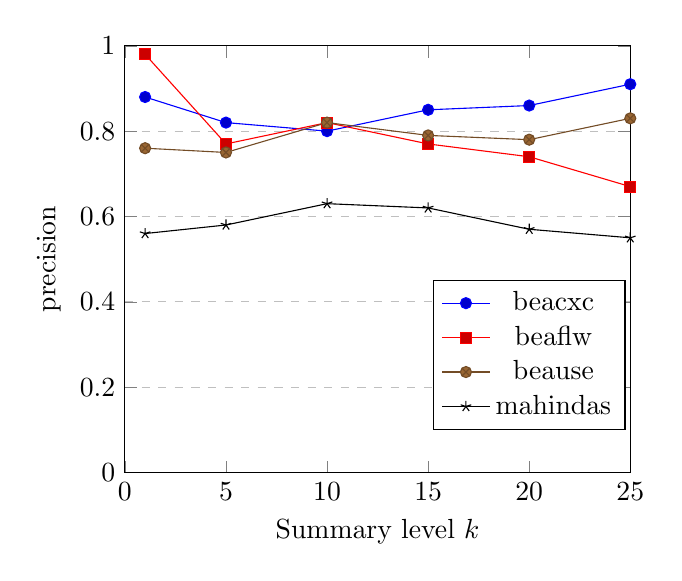
\begin{tikzpicture}
        \begin{axis}[
            xlabel={Summary level $k$},
            ylabel={precision},
            xmin=0, xmax=25,
            ymin=0, ymax=1.0,
            xtick={0,5,10,15,20,25},
            ymajorgrids=true,
            grid style=dashed,
            legend style={at={(0.8,0.1)},anchor=south},
            width=8cm,height=7cm]

            \addplot coordinates {
                (1,0.88)(5,0.82)(10,0.8)(15,0.85)(20,0.86)(25,0.91)
            };
            \addlegendentry{beacxc}
            
            \addplot coordinates {
                (1,0.98)(5,0.77)(10,0.82)(15,0.77)(20,0.74)(25,0.67)
            };
            \addlegendentry{beaflw}
        
            \addplot coordinates {
                (1,0.76)(5,0.75)(10,0.82)(15,0.79)(20,0.78)(25,0.83)
            };
            \addlegendentry{beause}
        
            \addplot coordinates {
                (1,0.56)(5,0.58)(10,0.63)(15,0.62)(20,0.57)(25,0.55)
            };
            \addlegendentry{mahindas}
        \end{axis}
    \end{tikzpicture}
    \caption{}
    %\caption{Precision of functional clusters generated by adapted FUSE algorithm}
    \label{fig:Precision}
\end{subfigure}

\begin{subfigure}[pt]{0.45\linewidth}
    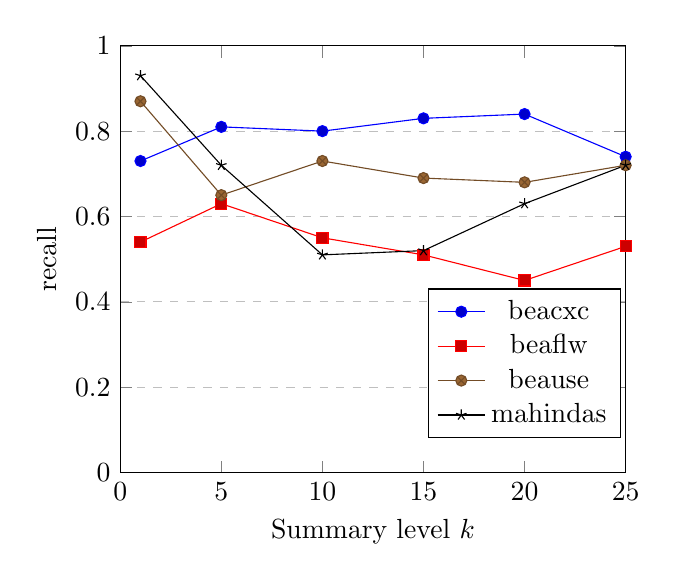
\begin{tikzpicture}
        \begin{axis}[
            xlabel={Summary level $k$},
            ylabel={recall},
            xmin=0, xmax=25,
            ymin=0, ymax=1.0,
            xtick={0,5,10,15,20,25},
            ymajorgrids=true,
            grid style=dashed,
            legend style={at={(0.8,0.08)},anchor=south},
            width=8cm,height=7cm]

            \addplot coordinates {
                (1,0.73)(5,0.81)(10,0.8)(15,0.83)(20,0.84)(25,0.74)
            };
            \addlegendentry{beacxc}
            
            \addplot coordinates {
                (1,0.54)(5,0.63)(10,0.55)(15,0.51)(20,0.45)(25,0.53)
            };
            \addlegendentry{beaflw}
        
            \addplot coordinates {
                (1,0.87)(5,0.65)(10,0.73)(15,0.69)(20,0.68)(25,0.72)
            };
            \addlegendentry{beause}
        
            \addplot coordinates {
                (1,0.93)(5,0.72)(10,0.51)(15,0.52)(20,0.63)(25,0.72)
            };
            \addlegendentry{mahindas}
        \end{axis}
    \end{tikzpicture}
    \caption{}
    %\caption{Recall of generated functional clusters from adapted FUSE algorithm}
    \label{fig:Recall}
\end{subfigure}
}


\caption{Cluster quality obtained using the adapted FUSE algorithm to summarize KGs from the financial sector. (a) Precision values. (b) Recall values}
\label{fig:ClustersQuality}
\end{figure*}


\begin{figure*}[!h]
\centering
\resizebox{2\columnwidth}{!}{
\begin{subfigure}[pt]{0.45\linewidth}
    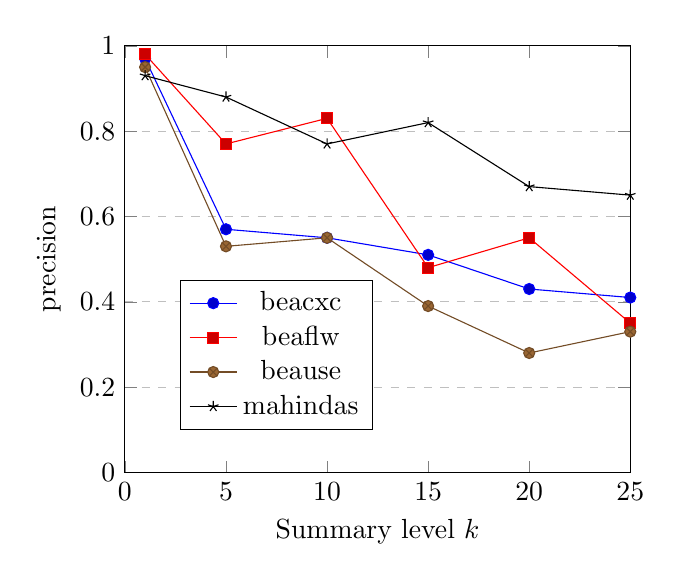
\begin{tikzpicture}
        \begin{axis}[
            xlabel={Summary level $k$},
            ylabel={precision},
            xmin=0, xmax=25,
            ymin=0, ymax=1.0,
            xtick={0,5,10,15,20,25},
            ymajorgrids=true,
            grid style=dashed,
            legend style={at={(0.3,0.1)},anchor=south},
            width=8cm,height=7cm]

            \addplot coordinates {
                (1,0.97)(5,0.57)(10,0.55)(15,0.51)(20,0.43)(25,0.41)
            };
            \addlegendentry{beacxc}
            
            \addplot coordinates {
                (1,0.98)(5,0.77)(10,0.83)(15,0.48)(20,0.55)(25,0.35)
            };
            \addlegendentry{beaflw}
        
            \addplot coordinates {
                (1,0.95)(5,0.53)(10,0.55)(15,0.39)(20,0.28)(25,0.33)
            };
            \addlegendentry{beause}
        
            \addplot coordinates {
                (1,0.93)(5,0.88)(10,0.77)(15,0.82)(20,0.67)(25,0.65)
            };
            \addlegendentry{mahindas}
        \end{axis}
    \end{tikzpicture}
    \caption{}
    %\caption{Precision of clusters generated the graph-based $k-means$ algorithm}
    \label{fig:Precision}
\end{subfigure}

\begin{subfigure}[pt]{0.45\linewidth}
    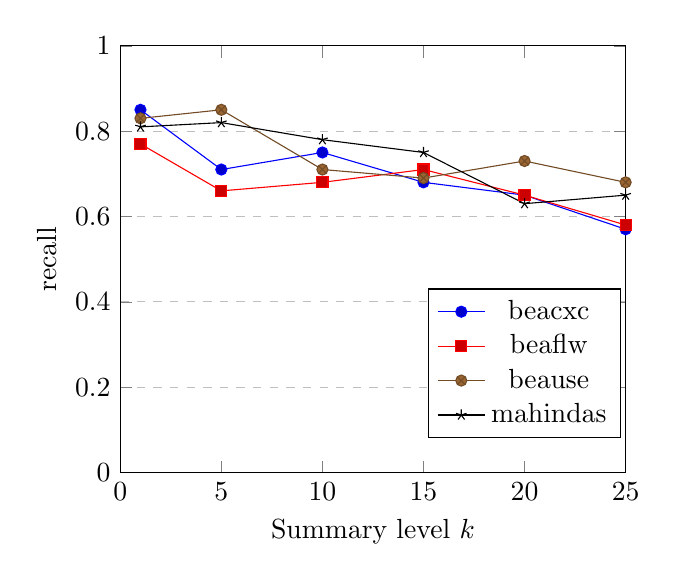
\begin{tikzpicture}
        \begin{axis}[
            xlabel={Summary level $k$},
            ylabel={recall},
            xmin=0, xmax=25,
            ymin=0, ymax=1.0,
            xtick={0,5,10,15,20,25},
            ymajorgrids=true,
            grid style=dashed,
            legend style={at={(0.8,0.08)},anchor=south},
            width=8cm,height=7cm]

            \addplot coordinates {
                (1,0.85)(5,0.71)(10,0.75)(15,0.68)(20,0.65)(25,0.57)
            };
            \addlegendentry{beacxc}
            
            \addplot coordinates {
                (1,0.77)(5,0.66)(10,0.68)(15,0.71)(20,0.65)(25,0.58)
            };
            \addlegendentry{beaflw}
        
            \addplot coordinates {
                (1,0.83)(5,0.85)(10,0.71)(15,0.69)(20,0.73)(25,0.68)
            };
            \addlegendentry{beause}
        
            \addplot coordinates {
                (1,0.81)(5,0.82)(10,0.78)(15,0.75)(20,0.63)(25,0.65)
            };
            \addlegendentry{mahindas}
        \end{axis}
    \end{tikzpicture}
    \caption{}
    %\caption{Recall of generated clusters generated by the graph-based $k-means$ algorithm}
    \label{fig:Recall}
\end{subfigure}
}


\caption{Cluster quality obtained using the graph-based $k-means$ algorithm to summarize KGs from the financial sector. (a) Precision values. (b) Recall values}
\label{fig:ClustersQualityClassical}
\end{figure*}

\textbf{Define a subset of visual data exploration tasks}
The following three tasks associated with the decision-making 
process in the financial sector are selected to conduct
the usability assessment:

\begin{enumerate}
    \item \textbf{FIBO01}: Observe the neighbors of the \textit{mean} term.
    \item \textbf{FIBO02}: Observe the relationships associated with the \textit{geopolitical entity} node. 
    \item \textbf{FIBO03}: Identify two types of relationships.
\end{enumerate}

\textbf{Select a group of analysts}. The tasks mentioned above were performed by
two analysts familiarized with graphs concepts and exploratory data analysis.

\textbf{Fix the layout algorithm}. The algorithm selected to generate the layout of the 
analyzed summary is the Fruchterman-Reingold algorithm.

\subsubsection{Analyze visual data exploration tasks}
\textbf{Measure time to complete every task}
As it is suggested in \cite{Camarillo20}, the efficiency of the obtained visual representation 
is measured by recording the analysis session where every user completes the visual exploration
tasks. After completing each task, the recording is stopped and the duration of this video represents
the value of the time needed to compute the efficiency metric. The efficiency of the visual 
representation is computed using the following formula:

\begin{equation}
  Efficiency = \frac{\sum_{j=1}^{R} \sum_{i=1}^{N} \frac{n_{ij}}{t_{ij}}}{NR}
  \label{eq:Efficiency}
\end{equation}

Where N is the number of tasks, R is the number of users, if the user
successfully completes the $i-th$ task $n_{ij} = 1$ otherwise  $n_{ij} = 0$
and $t_{ij}$ represents the time spent by $j-th$ user to complete the $i-th$
task. In Figure \ref{fig:Efficiency}, the visualized clustering result is 
16\% less efficiency for tasks \textbf{FIBO02} and \textbf{FIBO03}
compared with task \textbf{FIBO01}.

\begin{figure}[ht]
    \centering
    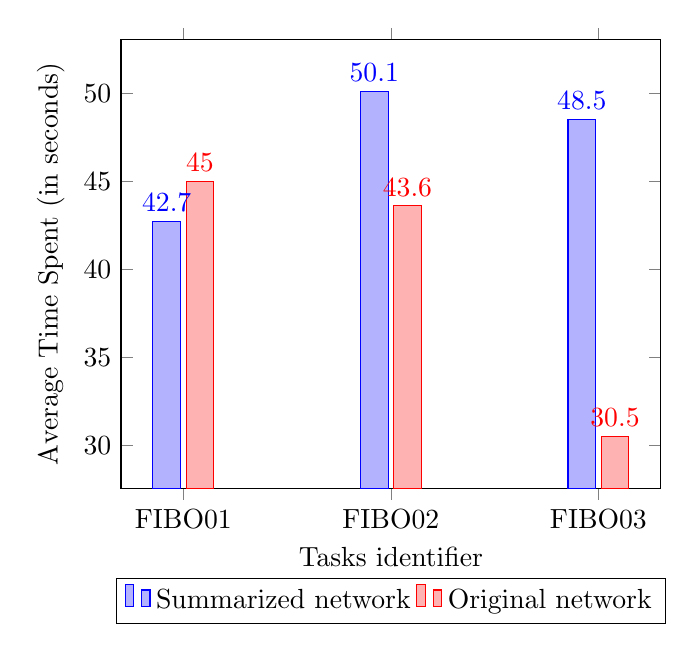
\begin{tikzpicture}
    \begin{axis}[
    ybar,
    enlargelimits=0.15,
    ylabel={Average Time Spent (in seconds)},
    xlabel={Tasks identifier},
    legend style={at={(0.5,-0.2)},
    anchor=north,legend columns=-1},
    %width=0.8*\textwidth,
    %height=9cm,
    %bar width=40pt,
    symbolic x coords={FIBO01,FIBO02,FIBO03},
    xtick=data,
    nodes near coords,
    nodes near coords align={vertical}
    ]
            \addplot
            coordinates {(FIBO01,42.7) (FIBO02,50.1) (FIBO03,48.5)};
            
            \addplot
            coordinates {(FIBO01,45.0) (FIBO02,43.6) (FIBO03,30.5)};
            
            \legend{Summarized network, Original network}
        \end{axis}
    \end{tikzpicture}
    \caption{Efficiency of visual data exploration tasks performed on functional summaries}
    \label{fig:Efficiency}
\end{figure}

\subsection{Discussion}

The modified FUSE algorithm suggests that the summary level 
do not affect precision values. For \textit{beacxc} and \textit{beause}
datasets, precision reaches 0.82 when summary level is $k = 25$. The
only network in which precision decreases when the summary level is increased
is \textit{beaflw}, falling out to 0.76 when $k = 25$. The lowest precision was
observed for the clusters computed for the \textit{mahindas} network, which barley 
exceeds 0.6 for $k = 10$ and $k = 15$. Precision values of the modified FUSE algorithm
are better than the precision values obtained
with the $k-means$ algorithm. With $k = 25$, the maximum precision value for $k-means$
clustering is 0.65, which is the barley greater than the minimum precision value obtained
by the adapted FUSE algorithm.

On the other hand, recall values show a poor quality for clusters computed when the
level of summary is increased compared with the $k-means$ clustering strategy. For \textit{beaflw} 
network, the recall value is 0.54 when the summary level is $k = 1$, when the summary level $k$
increases to $25$, this metric falls out to 0.53. In general, this pattern of
decreasing the recall value while the summary level increases occurs for 
the four summarized networks. In contrast, the recall values observed in
experiments with the $k-means$ clustering show a stability trend when the summary level increases. When
the summary level is 25, the minimum recall value is 0.57 ($beacxc$ network).

Regarding visual representation efficiency of the \textit{mahindas} network, the
user interface needs to be improved. The analysts that fulfill the visual 
exploration tasks using the summarized network invested more time than the 
time spent to perform the analysis tasks by visualizing the entire graph. For
a common task, such as \textbf{FIBO02}, users spent 50.1 seconds in average.
Future work is on improving the usability evaluation of the 
visualization systems that manage summarized networks due to the poor performance of the user interface.

\section{Conclusion}

In this paper an adaptation of the FUSE algorithm is utilized to summarize knowledge graphs. In order to generate the functional clusters, the structural knowledge information value is introduced as a parameter to determine whether a node from the original graph belongs or not to the initial clusters. Public data from the financial sector is used to validate the initial hypothesis of the applicability of the FUSE algorithm to generate functional clusters for different biology domains.  Then,  summarized networks are visualized and the efficiency of this visual representation is measured to evaluate the usability of functional clusters for exploratory data analysis tasks.


\bibliography{vis} 
\bibliographystyle{IEEEtran}
\EOD

\end{document}
